\section{System composition}
In this section, the different subsystems are elucidated, followed by how they are combined together to form the proposed architecture of the prototype.
\subsection{Subsystems}
\begin{itemize}
\item \textbf{VLC}
	\begin{itemize}
		\item LibVLC
		\item LibVLCcore
		\item VLC modules
		\item Buffer
		\item VLC media player
	\end{itemize}
\item \textbf{Tribler}
	\begin{itemize}
		\item Core
		\item Video Player control
		\item Libtorrent
	\end{itemize}
\item \textbf{GUI}
	\begin{itemize}
		\item start 
		\item VLC media player
	\end{itemize}
\end{itemize}
\subsection{Composition}
In figure \ref{fig:prop_arch} a visual overview of the proposed architecture can be found. In this figure, the different subsystem are combined in to one system.
\pagebreak
\pagebreak
\begin{figure}[h]
	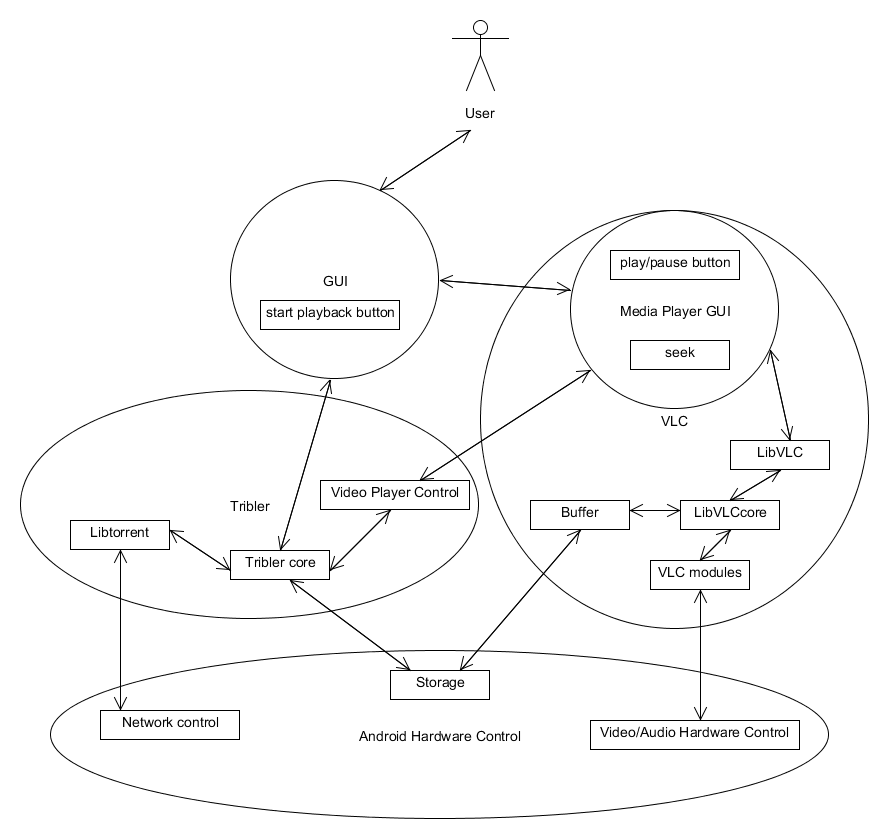
\includegraphics[scale=0.47]{images/architecture_overview.pdf}
	\caption{The proposed architecture of the prototype}
	\label{fig:prop_arch}
\end{figure}
\pagebreak